% == FG VC => Seq Comp ==
\section{Fine-Grained Protocols}

\begin{frame}{Two Perspectives on Fine-Grained Protocols}
	
	\begin{itemize}
		\item Cryptographic Perspective
		\item  Rational Perspective
	\end{itemize}
\end{frame}

\begin{frame}[t]{Crypto Perspective}
	\textit{A FG protocol is one secure against a specific complexity class $\class{C}$}.\pause\\
	\bigskip
\textit{Examples in literature:}
	\begin{itemize}
		\item Key-Exchange secure against $o(n^2)$ advs \cite{merkle}. \pause
		\item Key-Exchange and Symm. Key secure against space-bounded advs \cite{maurer}.\pause 
		\item Public-Key Encryption secure against $\NC^1$ advs \cite{fgcrypto} under $\L \not = \NC^1$.
	\end{itemize}
\end{frame}

\begin{frame}[t]{Rational Perspective}
\textit{In a FG protocol cheating costs strictly more than acting honestly.}\pause\\\medskip

\begin{block}{Theorem}
	A FG Verifiable Computation scheme yields a sequentially composable rational proof.
\end{block}
\onslide<3->
\begin{columns}
	\column{0.5\textwidth}
	\begin{figure}
		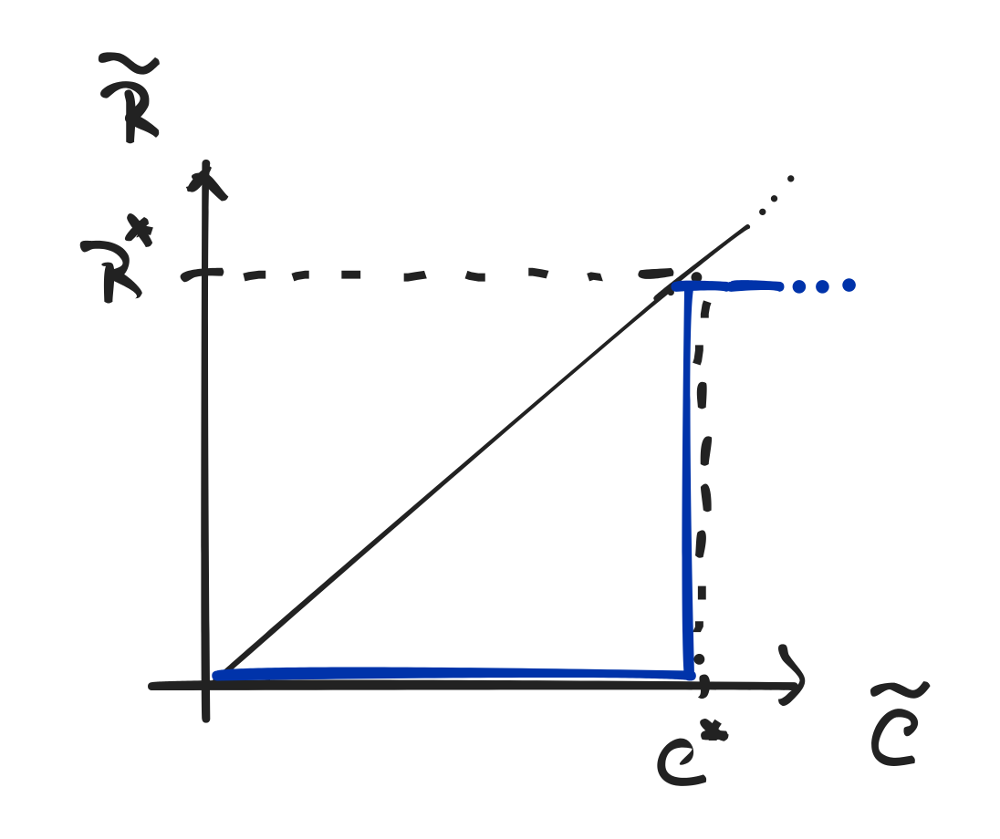
\includegraphics[scale=0.14]{pics/fg-sc.png}
		\caption{Cost/Reward in a FG protocol; V pays $R^*$ if she accepts}
	\end{figure}
	\onslide<4->
	\column{0.5\textwidth}
		\begin{figure}
			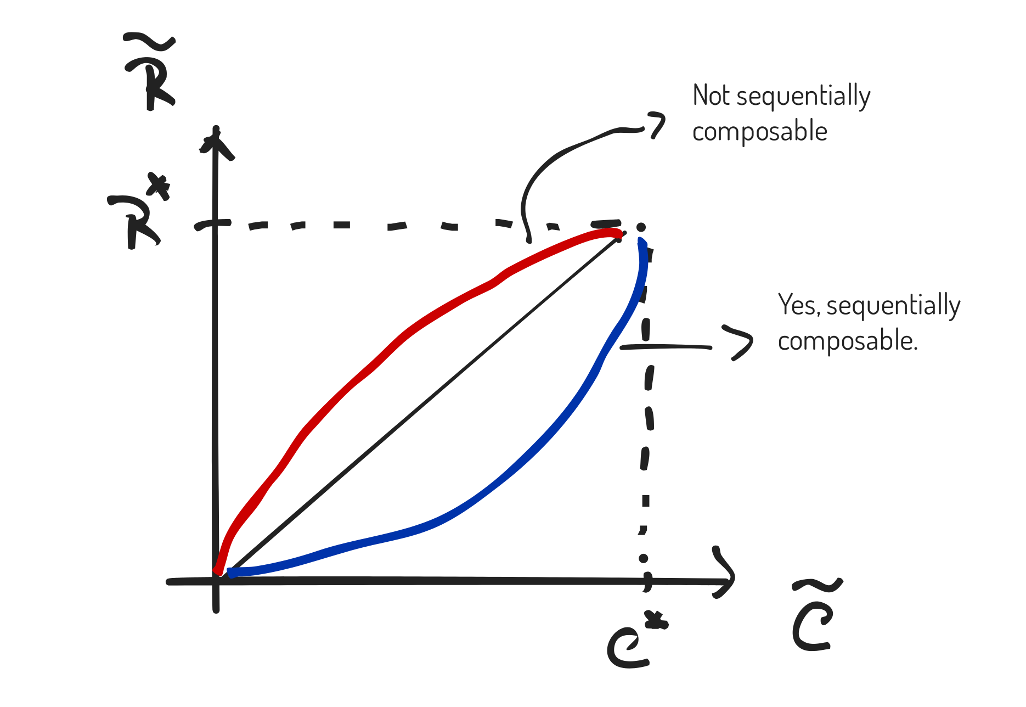
\includegraphics[scale=0.15]{pics/sc-char.png}
			\caption{Sequentially Composability (characterization)}
		\end{figure}
			
\end{columns}
\end{frame}

% == Our main result: FG VC against NC1 adversaries from minimal assumptions ==
\begin{frame}{Our FG Verifiable Computation Scheme}

\begin{block}{Our Main Result}
	A Non-Interactive Verifiable Computation Scheme secure against $\NC^1$ under $\L \not = \NC^1$.
\end{block}
\pause
\textbf{Properties:}
\begin{itemize}[<+- | alert@+>]
	\item I/O private;
	\item Reusable (in the preprocessing model);
	\item Supports delegation of (a subset of) $\ACzt$.
\end{itemize}
\pause
\bigskip
\hrule
\medskip
\begin{columns}
	\column{0.33\textwidth}
	$\NC^1: $ log-depth, fan-in two.\\\vspace{1cm}
	\pause
	\column{0.33\textwidth}
	$\AC^0: $ constant-depth, unbounded fan-in, AND/OR/NOT gates.\\\vspace{1cm}
	\pause
	\column{0.33\textwidth}
		$\ACzt: \AC^0 + $  XOR gates.\\\vspace{1cm} \pause
		$\AC^0 \subsetneq \ACzt \subsetneq \NC^1$ 
\end{columns}
\end{frame}


% == How to obtain this VC: HE + transformation ==
% Say here that another result will be for HE
\begin{frame}{How We Obtain Fine-Grained VC}
	Core of our approach is \cite{ckv10}:
	\begin{itemize}
		\item  Obtains VC from Homomorphic Encryption (HE)
	\end{itemize}
\end{frame}

\def\E{\func{E}}

% == Homomorphic Encryption ==
\begin{frame}{Homomorphic Encryption (HE)}
	\begin{center} \textbf{HE = PKE + Evaluation Function} \end{center}
	\pause
	\begin{enumerate}
		\item $\func{KeyGen} \to (\pk, \sk)$
		\item $\func{Enc}_{\pk}(x) \to \E(x)$
		\item $\func{Dec}_{\sk}(\E(x)) \to x$
		\pause  
		\item $\func{Eval}_{\pk}(f, \E(x)) \to \E(f(x))$
	\end{enumerate}
	\pause
	\bigskip
	\begin{block}{Our Additional Result}
		HE secure against $\NC^1$ adversaries under $\L \not = \NC^1$ and supporting evaluation of (a subset of) $\ACzt$.
	\end{block}
\end{frame}

% == VC from HE ==
\begin{frame}[t]{Our Starting Point: VC from HE (\cite{ckv10})}
%	\begin{framed}
%	Core of our approach is \cite{ckv10}:
%	\begin{itemize}
%		\item  Obtains VC from Homomorphic Encryption (HE)
%	\end{itemize}
%	\end{framed}
%	\pause
	\onslide<2->
\begin{columns}
		\column{0.65\textwidth}
	\procedure{Protocol from \cite{ckv10}}{%
		\textbf{Delegator} \> \> \textbf{Worker}  \\
		%r \sample \bin^n\\
		\vect{c}_0 \gets \E(0) \\
		\vect{y^*_0} \gets \func{Eval}(f, \vect{c}_0)\pclb
		\pcintertext[dotted]{End Offline Stage}
		\vect{c}_1 \gets \E(x)\\
		b \sample \bin \> \> \\
		\> \xrightarrow{\vect{c}_b, \vect{c}_{1-b}} \>  \\
		\> \> \vect{y}_0 \gets \func{Eval}(f, \vect{c}_0)    \\
		\> \> \vect{y}_1 \gets \func{Eval}(f, \vect{c}_1)    \\
		\> \xleftarrow{\vect{y}_b,\vect{y}_{1-b}} \>   \\
		\text{accept } \func{Dec}(\vect{y}_1) \text{ if } \vect{y}_0 = \vect{y^*_0} \> \>}
	\onslide<3->
	\column{0.35\textwidth}
	\textbf{Then:}
	\begin{itemize}
		% TODO: Improve graphics so that changes are clear
		\item \textbf{To amplify error:} use random permutation;
			\onslide<4->
		\item \textbf{To make reusable:} use HE  on top of construction.
	\end{itemize}
	
	\end{columns}
	% Scaling this up: error amplification (permutation); reusability
\end{frame}


% == VC from HE in low depth ==
\begin{frame}[t]{Challenge: Ensuring \cite{ckv10} Works in Low-Depth}
	\textbf{Recall:} all our algorithms should run in $\NC^1$ and our verifier should be efficient.\pause\\
	\bigskip
	\textbf{Some of the issues to take care of: }
	\begin{itemize}[<+- | alert@+>]
		\item How can we sample a random permutation in sufficiently low-depth?
		\item When using ``double'' HE, does double evaluation stay in $\NC^1$?
%		\item How to make sure it works when HE has \textit{randomized} decryption? (our decryption is randomized, but the original construction only works for deterministic)
		\item In the proof, does the security reduction stay in $\NC^1$?
	\end{itemize}
\end{frame}

% == HE against NC1 circuits==
\begin{frame}[t]{Obtaining HE Secure Against $\NC^1$ Adversaries}
\begin{block}{Recall Our Additional Result:}
	HE against secure against $\NC^1$ adversaries under $\L \not = \NC^1$ supporting evaluation of (a subset of) $\ACzt$.
\end{block}
\pause
\bigskip
	\textbf{Our Approach (sketch):}
	\begin{enumerate}[<+- | alert@+>]
		\item We start from the PKE secure against $\NC^1$ in \cite{fgcrypto};
		\item We apply relinearization techniques from \cite{fhe-lwe} to obtain somewhat HE;
		\begin{itemize}
			\item Can homomorphically evaluate polynomials of constant degree; 
		\end{itemize}
		\item We extend the class of functions we can evaluate homomorphically through degree reduction techniques from \cite{razborov1987lower}.
	\end{enumerate}%\pause
	%\textbf{Next, we see 1 and 2.}
\end{frame}

\begin{frame}{Comparison with Prior Work}
	Comparison with information-theoretic results:
	\begin{itemize}[<+- | alert@+>]
		\item ``Proofs for Muggles'' \cite{muggles} obtains constant-round protocols for $\NC^1$.
		\begin{itemize}
			\item results in \cite{muggles} hold unconditionally; 
			\item our verifier runs in $\ACzt$; theirs in $\TC^0$;
			\item our protocol is I/O private and non-interactive.
		\end{itemize}
		\item \cite{gghkr07} obtains constant-depth ($\NC^0$) protocols for $\NC^1$.
		\begin{itemize}
			\item large verifier ($n^3$) and communication overhead.
		\end{itemize}
	\end{itemize}
\end{frame}
